\documentclass[a4paper,12pt]{article}

\usepackage{graphicx}
\usepackage{wrapfig}
\usepackage{amsmath}
\usepackage{amsfonts}
\usepackage[english, russian]{babel}
\usepackage[T1, T2A]{fontenc}
\usepackage[utf8]{inputenc}
\usepackage{geometry}
\usepackage{indentfirst}
\usepackage{listings}
\usepackage[dvipsnames]{xcolor}
\usepackage[colorlinks]{hyperref}
\usepackage{amsmath}
\graphicspath{ {./images/} }
\geometry{left=2cm, right=2cm, bottom=2cm, top=2cm}

\hypersetup{
    linkcolor=blue,
    filecolor=magenta,
    urlcolor=cyan
}

\lstset{
    backgroundcolor=\color{white},
    basicstyle=\footnotesize\ttfamily,
    breaklines=true,
    frame=single,
    numbers=left,
    numberstyle=\tiny\color{gray},
    keywordstyle=\color{blue},
    commentstyle=\color{green!40!black},
    stringstyle=\color{darkblue},
    showstringspaces=false,
    tabsize=4,
    language=Mathematica
}

\definecolor{codegreen}{rgb}{0,0.6,0}
\definecolor{codegray}{rgb}{0.5,0.5,0.5}
\definecolor{codepurple}{rgb}{0.58,0,0.82}
\definecolor{backcolour}{rgb}{0.95,0.95,0.92}


\lstdefinestyle{codestyle}{
    backgroundcolor=\color{backcolour},
    commentstyle=\color{codegreen},
    keywordstyle=\color{blue},
    numberstyle=\tiny\color{codegray},
    stringstyle=\color{magenta},
    basicstyle=\ttfamily\footnotesize,
    breakatwhitespace=false,
    breaklines=true,
    captionpos=b,
    keepspaces=true,
    numbers=left,
    numbersep=5pt,
    showspaces=false,
    showstringspaces=false,
    showtabs=false,
    tabsize=2
}













\lstset{style=codestyle}
\lstset{extendedchars=\true}

\begin{document}
\begin{titlepage}
    \centering
    \vspace*{1cm}

    {\large Министерство науки и высшего образования Российской Федерации}\\
    {\large ФЕДЕРАЛЬНОЕ ГОСУДАРСТВЕННОЕ АВТОНОМНОЕ ОБРАЗОВАТЕЛЬНОЕ УЧРЕЖДЕНИЕ ВЫСШЕГО ОБРАЗОВАНИЯ «НАЦИОНАЛЬНЫЙ ИССЛЕДОВАТЕЛЬСКИЙ УНИВЕРСИТЕТ ИТМО»}\\
    {\large (УНИВЕРСИТЕТ ИТМО)}\\

    \vspace{2cm}

    {\large Факультет «Систем управления и робототехники»}\\

    \vspace{3cm}

    \textbf{{\Huge ОТЧЕТ}\\
    {\Huge О ЛАБОРАТОРНОЙ РАБОТЕ №2}}\\

    \vspace{1cm}

    {\LARGE По дисциплине «Частотные методы»}\\
    {\LARGE на тему: «Преобразования фурье»}\\

    \vspace{3cm}

    {\Large Студент:}\\
    Охрименко Ева

    \vspace{2cm}

    {\Large Преподаватели:}\\
    Догадин Егор Витальевич\\
    Пашенко Артем Витальевич\\

    \vspace{3cm}
    {\large г. Санкт-Петербург}\\
    {\large 2025}

\end{titlepage}
\newpage
\tableofcontents
\newpage


\section{Вещественное задание}
\subsection{Краткое условие}
Для каждой из функций \( f(t) \) провести исследование её Фурье-образа \(\hat{f}(\omega)\):

\begin{itemize}
    \item Привести аналитические выражения для \( f(t) \) и \(\hat{f}(\omega)\).
    \begin{itemize}
        \item Для прямоугольной, треугольной и двустороннего затухания функций — с выкладками.
        \item Для кардинального синуса и функции Гаусса — только результат.
    \end{itemize}

    \item Выбрать три набора значений \( a, b > 0 \).

    \item Построить графики \( f(t) \) и \(\hat{f}(\omega)\) для выбранных параметров.

    \item Проверить равенство Парсеваля.

    \item Сделать выводы о влиянии параметров \( a \) и \( b \).
\end{itemize}

\subsection{Прямоугольная функция}
\subsubsection{Аналитика}
Исходная функция:
\[
f(t) = 
\begin{cases} 
a, & |t| \leq b, \\
0, & |t| > b.
\end{cases}
\]

Фурье-образ вычисляется по формуле:
\[
\hat{f}(\omega) = \frac{1}{\sqrt{2\pi}} \int_{-b}^{b} a e^{-i\omega t} dt = \frac{a}{\sqrt{2\pi}} \left[ \frac{e^{-i\omega t}}{-i\omega} \right]_{-b}^{b} = \frac{a}{\sqrt{2\pi}} \cdot \frac{e^{-i\omega b} - e^{i\omega b}}{-i\omega} = \frac{a}{\sqrt{2\pi}} \cdot \frac{-2i \sin(\omega b)}{-i\omega} = \frac{2a \sin(\omega b)}{\omega \sqrt{2\pi}}.
\]

Таким образом, Фурье-образ прямоугольной функции:
\[
\hat{f}(\omega) = \frac{2a \sin(\omega b)}{\omega \sqrt{2\pi}}.
\]


Для параметров \( (a, b) = (1, 1) \):
\[
\hat{f}(\omega) = \sqrt{\frac{2}{\pi}} \cdot \frac{\sin(\omega)}{\omega}.
\]

Для параметров \( (a, b) = (2, 2) \):
\[
\hat{f}(\omega) = 2 \sqrt{\frac{2}{\pi}} \cdot \frac{\sin(2\omega)}{\omega}.
\]

Для параметров \( (a, b) = (5, 4) \):
\[
\hat{f}(\omega) = 5 \sqrt{\frac{2}{\pi}} \cdot \frac{\sin(4\omega)}{\omega}.
\]

\subsubsection{Код}
\begin{lstlisting}[caption=Фурье-образ прямоугольной функции и проверка равенства Парсеваля]
f[t_,a_,b_]:=Piecewise[{{a,Abs[t]<=b},{0,Abs[t]>b}}]

a=1;
b=1;

fourier=FourierTransform[f[t,a,b],t,w]

Plot[f[t,a,b],{t,-5,5},PlotRange->All,PlotStyle->Thick,AxesLabel->{"t","f(t)"},PlotLabel->"Прямоугольная функция",Exclusions->None]

Plot[Re[fourier],{w,-10,10},PlotRange->All,PlotStyle->Thick,AxesLabel->{"\[Omega]","F(\[Omega])"},PlotLabel->"Фурье-образ прямоугольной функции"]

energyTimeDomain = Integrate[Abs[f[t, a, b]]^2, {t, -Infinity, Infinity}];

energyFrequencyDomain = Integrate[Abs[fourier]^2, {w, -Infinity, Infinity}];

Print["\nПроверка равенства Парсеваля:"]
Print["\[Integral]|f(t)|\.b2 dt = ", energyTimeDomain]
Print["\[Integral]|F(\[Omega])|\.b2 d\[Omega] = ", energyFrequencyDomain]
Print["Результат: ", energyTimeDomain == energyFrequencyDomain]
\end{lstlisting}
Этот код определяет прямоугольную функцию, вычисляет её Фурье-образ, строит графики и проверяет равенство Парсеваля.

\subsubsection{Вывод}
Теперь посмотрим на вывод кода. Я построю графики прямоугольной функции и Фурье-образа для выбранных значений.
\begin{center}
\begin{minipage}{0.48\textwidth}
  \centering
  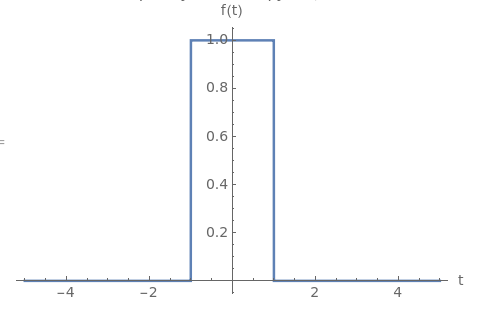
\includegraphics[width=\linewidth]{images/1f11.png}
  \captionof{\( f(t) \) для \( (a, b) = (1, 1) \) .}
\end{minipage}
\hfill
\begin{minipage}{0.48\textwidth}
  \centering
  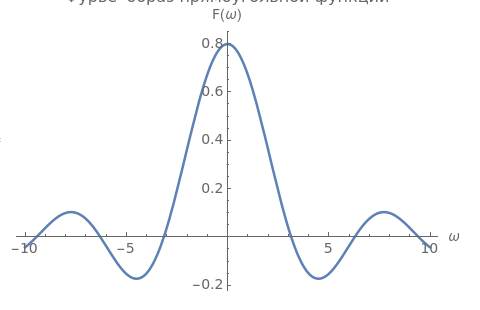
\includegraphics[width=\linewidth]{images/1F11.png}
  \captionof{\( \hat{f}(\omega) \) для \( (a, b) = (1, 1) \).}
\end{minipage}
\end{center}


\begin{center}
\begin{minipage}{0.48\textwidth}
  \centering
  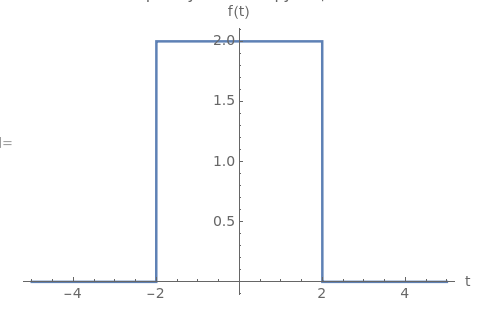
\includegraphics[width=\linewidth]{images/1f22.png}
  \captionof{\( f(t) \) для \( (a, b) = (2, 2) \) .}
\end{minipage}
\hfill
\begin{minipage}{0.48\textwidth}
  \centering
  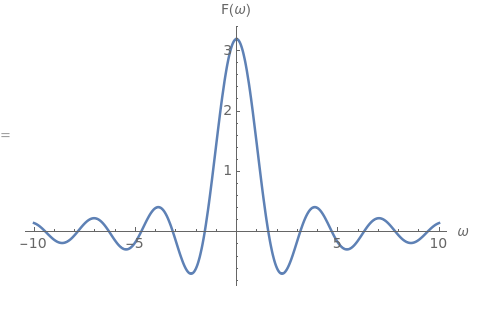
\includegraphics[width=\linewidth]{images/1F22.png}
  \captionof{\( \hat{f}(\omega) \) для \( (a, b) = (2, 2) \).}
\end{minipage}
\end{center}


\begin{center}
\begin{minipage}{0.48\textwidth}
  \centering
  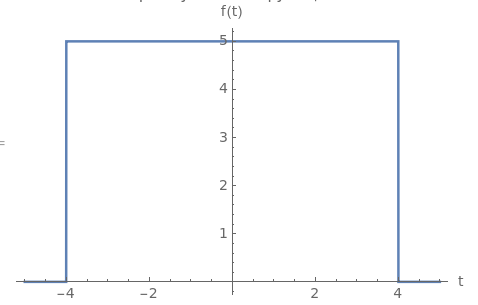
\includegraphics[width=\linewidth]{images/1f54.png}
  \captionof{\( f(t) \) для \( (a, b) = (5, 4) \) .}
\end{minipage}
\hfill
\begin{minipage}{0.48\textwidth}
  \centering
  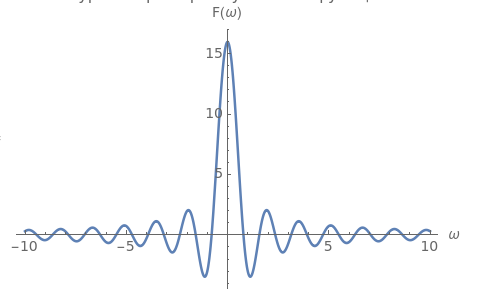
\includegraphics[width=\linewidth]{images/1F54.png}
  \captionof{\( \hat{f}(\omega) \) для \( (a, b) = (5, 4) \).}
\end{minipage}
\end{center}



Параметры \( a \) и \( b \) определяют форму прямоугольной функции и её Фурье-образ. В исходной функции \( b \) задаёт длину прямоугольника, а \( a \) — его высоту. При увеличении \( a \) амплитуда Фурье-образа возрастает, так как преобразование Фурье линейно, и умножение функции на константу \( a \) приводит к пропорциональному увеличению её Фурье-образа.

При увеличении \( b \) прямоугольник становится длиннее, что приводит к более "частым" и "узким" колебаниям в Фурье-образе. Это происходит из-за того, что преобразование Фурье сохраняет энергию сигнала, и увеличение ширины прямоугольника во временной области вызывает сжатие его спектра в частотной области.. \\


Также в моем коде присутствует проверка равенства Парсерваля. Для любых \( (a, b) \) проверка вернула \( True\) следовательно равенство выполнено.


\begin{center}
\begin{minipage}{0.32\textwidth}
  \centering
  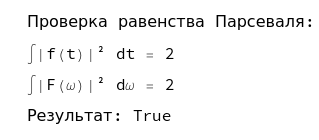
\includegraphics[width=\linewidth]{images/1P11.png}
  \captionof{\( (a, b) = (1, 1) \)}
\end{minipage}
\hfill
\begin{minipage}{0.32\textwidth}
  \centering
  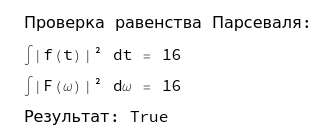
\includegraphics[width=\linewidth]{images/1P22.png}
  \captionof{\( (a, b) = (2, 2) \)}
\end{minipage}
\hfill
\begin{minipage}{0.32\textwidth}
  \centering
  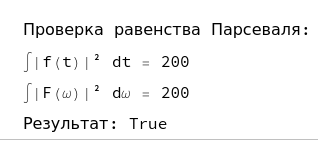
\includegraphics[width=\linewidth]{images/1P54.png}
  \captionof{\( (a, b) = (5, 4) \)}
\end{minipage}
\end{center}


\subsection{Треугольная функция}

\subsubsection{Аналитика}

Исходная функция:

\[
f(t) = 
\begin{cases} 
a - \left| \frac{a t}{b} \right|, & |t| \leq b, \\
0, & |t| > b.
\end{cases}
\]


Фурье-образ вычисляется по формуле:
\[
\hat{f}(\omega) = \frac{1}{\sqrt{2\pi}} \int_{-b}^{b} \left( a - \left| \frac{a t}{b} \right| \right) e^{-i\omega t} dt = \frac{a}{\sqrt{2\pi}} \left( \int_{0}^{b} \left( 1 - \frac{t}{b} \right) e^{-i\omega t} dt + \int_{-b}^{0} \left( 1 + \frac{t}{b} \right) e^{-i\omega t} dt \right) = \\
\]
\[
= \frac{a}{\sqrt{2\pi}} \left( \frac{e^{-i\omega b} - 1 + i\omega b}{b \omega^2} + \frac{1 + i\omega b - e^{i\omega b}}{b \omega^2} \right) = \frac{a}{\sqrt{2\pi}} \left( \frac{e^{-i\omega b} + e^{i\omega b} - 2}{b \omega^2} \right) = \frac{2a (1 - \cos(\omega b))}{\sqrt{2\pi} b \omega^2}
\]




Для параметров \( (a, b) = (1, 1) \):
\[
\frac{2 - 2 \cos (w)}{\sqrt{2 \pi w^2}}
\]

Для параметров \( (a, b) = (2, 2) \):
\[
\frac{4 - 4 \cos (2w)}{2\sqrt{2 \pi w^2}}
\]

Для параметров \( (a, b) = (5, 4) \):
\[
\frac{10 - 10 \cos (4w)}{4\sqrt{2 \pi w^2}}
\]


\subsubsection{Код}


\begin{lstlisting}[caption=Фурье-образ треугольной функции и проверка равенства Парсеваля]
f[t_, a_, b_] := 
 Piecewise[{{a - Abs[a t/b], Abs[t] <= b}, {0, Abs[t] > b}}]

a = 5;
b = 4;

fourier = FourierTransform[f[t, a, b], t, w]

Plot[f[t, a, b], {t, -5, 5}, PlotRange -> All, PlotStyle -> Thick, 
 AxesLabel -> {"t", "f(t)"}, PlotLabel -> "Треугольная функция"]

Plot[Re[fourier], {w, -10, 10}, PlotRange -> All, PlotStyle -> Thick, 
 AxesLabel -> {"\[Omega]", "F(\[Omega])"}, 
 PlotLabel -> "Фурье-образ треугольной функции"]

energyTimeDomain = 
  Integrate[Abs[f[t, a, b]]^2, {t, -Infinity, Infinity}];

energyFrequencyDomain = 
  Integrate[Abs[fourier]^2, {w, -Infinity, Infinity}];

Print["\nПроверка равенства Парсеваля:"]
Print["\[Integral]|f(t)|\.b2 dt = ", energyTimeDomain]
Print["\[Integral]|F(\[Omega])|\.b2 d\[Omega] = ", \
energyFrequencyDomain]
Print["Результат: ", energyTimeDomain == energyFrequencyDomain]
\end{lstlisting}
Этот код определяет треугольную функцию, вычисляет её Фурье-образ, строит графики и проверяет равенство Парсеваля.

\subsubsection{Вывод}
Теперь посмотрим на вывод кода. Я построю графики треугольной функции и Фурье-образа для выбранных значений.
\begin{center}
\begin{minipage}{0.48\textwidth}
  \centering
  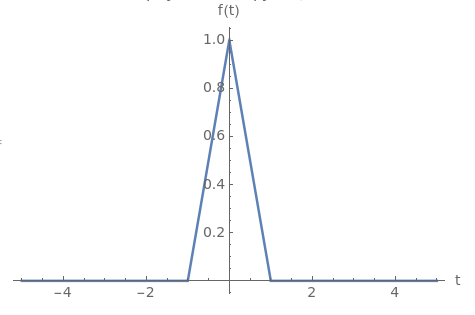
\includegraphics[width=\linewidth]{images/2f11.png}
  \captionof{\( f(t) \) для \( (a, b) = (1, 1) \) .}
\end{minipage}
\hfill
\begin{minipage}{0.48\textwidth}
  \centering
  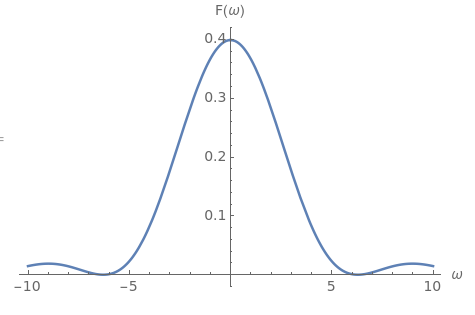
\includegraphics[width=\linewidth]{images/2F11.png}
  \captionof{\( \hat{f}(\omega) \) для \( (a, b) = (1, 1) \).}
\end{minipage}
\end{center}


\begin{center}
\begin{minipage}{0.48\textwidth}
  \centering
  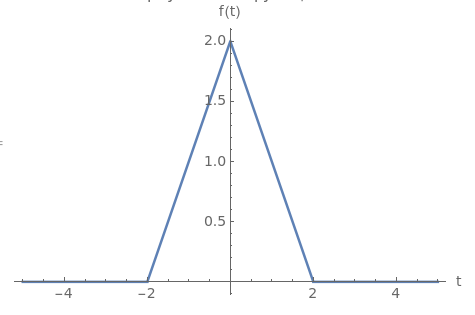
\includegraphics[width=\linewidth]{images/2f22.png}
  \captionof{\( f(t) \) для \( (a, b) = (2, 2) \) .}
\end{minipage}
\hfill
\begin{minipage}{0.48\textwidth}
  \centering
  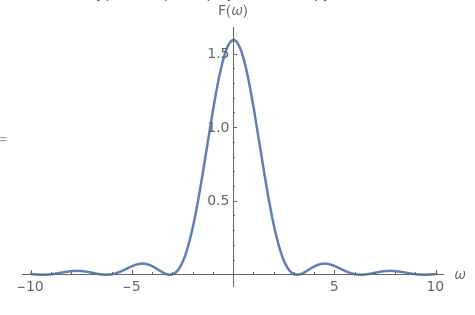
\includegraphics[width=\linewidth]{images/2F22.png}
  \captionof{\( \hat{f}(\omega) \) для \( (a, b) = (2, 2) \).}
\end{minipage}
\end{center}


\begin{center}
\begin{minipage}{0.48\textwidth}
  \centering
  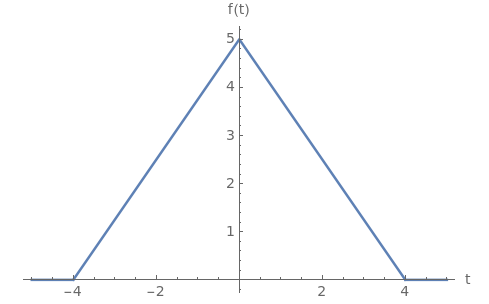
\includegraphics[width=\linewidth]{images/2f54.png}
  \captionof{\( f(t) \) для \( (a, b) = (5, 4) \) .}
\end{minipage}
\hfill
\begin{minipage}{0.48\textwidth}
  \centering
  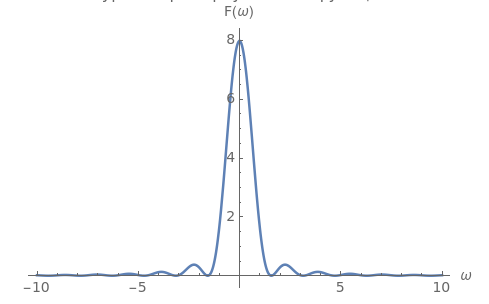
\includegraphics[width=\linewidth]{images/2F54.png}
  \captionof{\( \hat{f}(\omega) \) для \( (a, b) = (5, 4) \).}
\end{minipage}
\end{center}

Параметры \( a \) и \( b \) влияют на форму треугольной функции и её Фурье-образ. В исходной функции \( b \) задаёт ширину основания треугольника, а \( a \) — его высоту. При увеличении \( a \) амплитуда Фурье-образа увеличивается, потому что преобразование Фурье линейно, и умножение функции на константу \( a \) приводит к умножению её Фурье-образа на ту же константу.

При увеличении \( b \) основание треугольника становится шире, что приводит к более "частым" и "узким" колебаниям в Фурье-образе, потому что преобразование Фурье сохраняет энергию сигнала, и расширение во временной области компенсируется сжатием в частотной области. \\



Также в моем коде присутствует проверка равенства Парсерваля. Для любых \( (a, b) \) проверка вернула \( True\) следовательно равенство выполнено.

\begin{center}
\begin{minipage}{0.32\textwidth}
  \centering
  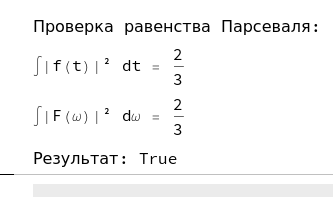
\includegraphics[width=\linewidth]{images/2P11.png}
  \captionof{\( (a, b) = (1, 1) \)}
\end{minipage}
\hfill
\begin{minipage}{0.32\textwidth}
  \centering
  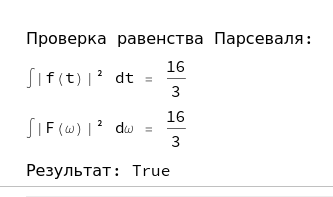
\includegraphics[width=\linewidth]{images/2P22.png}
  \captionof{\( (a, b) = (2, 2) \)}
\end{minipage}
\hfill
\begin{minipage}{0.32\textwidth}
  \centering
  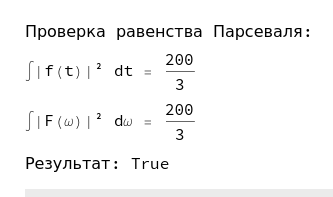
\includegraphics[width=\linewidth]{images/2P54.png}
  \captionof{\( (a, b) = (5, 4) \)}
\end{minipage}
\end{center}

\subsection{Кардинальный синус}
\subsubsection{Аналитика}
 Исходная функция
\[
f(t) = a \cdot \text{sinc}(b t) = a \cdot \frac{\sin(b t)}{b t}.
\]

Фурье-образ функции \( f(t) \):

\[
\hat{f}(\omega) = \int_{-\infty}^{\infty} f(t) e^{-i \omega t} \, dt = a \cdot \frac{\pi}{b} \cdot \text{rect}\left(\frac{\omega}{2 \pi b}\right),
\]

где \( \text{rect}(x) \) — прямоугольная функция, равная 1 при \( |x| \leq \frac{1}{2} \) и 0 в остальных случаях. 

\subsubsection{Код}
\begin{lstlisting}[caption=Фурье-образ кардинального синуса и проверка равенства Парсеваля]
f[t_, a_, b_] := a Sinc[b t]

a = 5;
b = 4;

fourier = FourierTransform[f[t, a, b], t, w]

Plot[f[t, a, b], {t, -10, 10}, PlotRange -> All, PlotStyle -> Thick, 
 AxesLabel -> {"t", "f(t)"}, 
 PlotLabel -> "Функция кардинального синуса"]

Plot[Re[fourier], {w, -10, 10}, PlotRange -> All, PlotStyle -> Thick, 
 AxesLabel -> {"\[Omega]", "F(\[Omega])"}, 
 PlotLabel -> "Фурье-образ функции кардинального синуса", 
 Exclusions -> None]

energyTimeDomain = 
 Integrate[Abs[f[t, a, b]]^2, {t, -Infinity, Infinity}]

energyFrequencyDomain = 
 Integrate[Abs[fourier]^2, {w, -Infinity, Infinity}]

Print["\nПроверка равенства Парсеваля:"]
Print["\[Integral]|f(t)|\.b2 dt = ", energyTimeDomain]
Print["\[Integral]|F(\[Omega])|\.b2 d\[Omega] = ", \
energyFrequencyDomain]
Print["Результат: ", energyTimeDomain == energyFrequencyDomain]
\end{lstlisting}
Этот код определяет функцию кардинального синуса, вычисляет его Фурье-образ, строит графики и проверяет равенство Парсеваля.

\subsubsection{Вывод}
Теперь посмотрим на вывод кода. Я построю графики кардинального и Фурье-образа для выбранных значений.
\begin{center}
\begin{minipage}{0.48\textwidth}
  \centering
  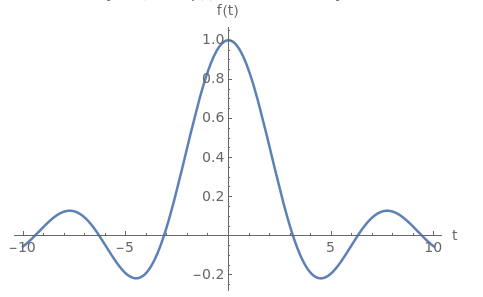
\includegraphics[width=\linewidth]{images/3f11.png}
  \captionof{\( f(t) \) для \( (a, b) = (1, 1) \) .}
\end{minipage}
\hfill
\begin{minipage}{0.48\textwidth}
  \centering
  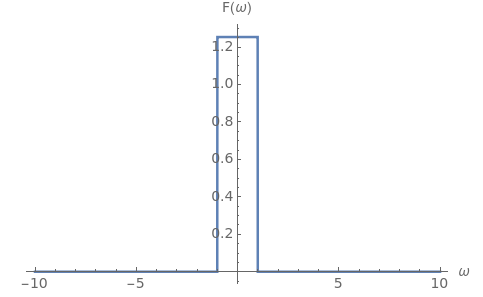
\includegraphics[width=\linewidth]{images/3F11.png}
  \captionof{\( \hat{f}(\omega) \) для \( (a, b) = (1, 1) \).}
\end{minipage}
\end{center}


\begin{center}
\begin{minipage}{0.48\textwidth}
  \centering
  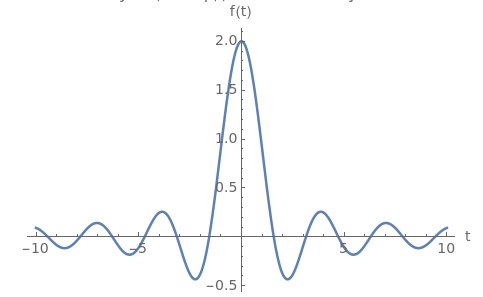
\includegraphics[width=\linewidth]{images/3f22.png}
  \captionof{\( f(t) \) для \( (a, b) = (2, 2) \) .}
\end{minipage}
\hfill
\begin{minipage}{0.48\textwidth}
  \centering
  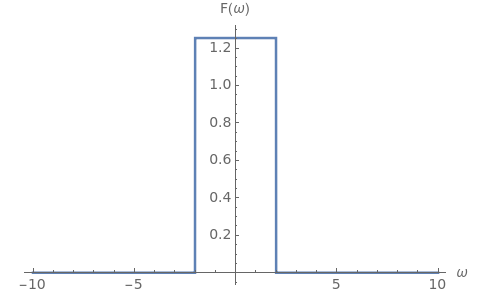
\includegraphics[width=\linewidth]{images/3F22.png}
  \captionof{\( \hat{f}(\omega) \) для \( (a, b) = (2, 2) \).}
\end{minipage}
\end{center}


\begin{center}
\begin{minipage}{0.48\textwidth}
  \centering
  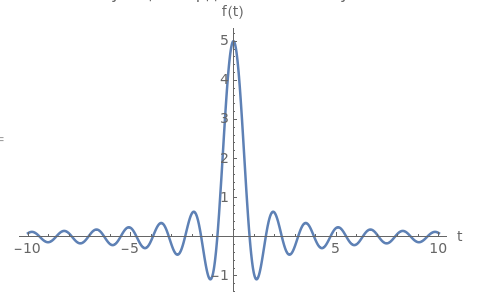
\includegraphics[width=\linewidth]{images/3f54.png}
  \captionof{\( f(t) \) для \( (a, b) = (5, 4) \) .}
\end{minipage}
\hfill
\begin{minipage}{0.48\textwidth}
  \centering
  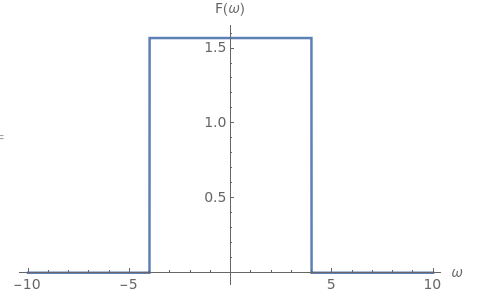
\includegraphics[width=\linewidth]{images/3F54.png}
  \captionof{\( \hat{f}(\omega) \) для \( (a, b) = (5, 4) \).}
\end{minipage}
\end{center}

Функция \( f(t) = a \cdot \text{sinc}(b t) \) имеет Фурье-образ, который определяется свойствами преобразования Фурье. Параметр \( a \) влияет на амплитуду функции и её Фурье-образа: при увеличении \( a \) амплитуда Фурье-образа увеличивается пропорционально, потому что преобразование Фурье линейно, и умножение функции на константу \( a \) приводит к умножению её Фурье-образа на ту же константу.

Параметр \( b \) влияет на масштабирование функции по оси времени: при увеличении \( b \) функция \( \text{sinc}(b t) \) становится более "сжатой" во временной области, потому что аргумент функции \( \text{sinc}(b t) \) увеличивается, что приводит к более быстрому затуханию колебаний. Это приводит к "растяжению" её Фурье-образа в частотной области, потому что преобразование Фурье сохраняет энергию сигнала, и сжатие во временной области компенсируется расширением в частотной области.

Таким образом, при увеличении \( b \) Фурье-образ становится более широким, потому что сжатие функции во временной области приводит к расширению её спектра в частотной области, а при уменьшении \( b \) — более узким, потому что расширение функции во временной области приводит к сжатию её спектра в частотной области.\\


Также в моем коде присутствует проверка равенства Парсерваля. Для любых \( (a, b) \) проверка вернула \( True\) следовательно равенство выполнено.

\begin{center}
\begin{minipage}{0.32\textwidth}
  \centering
  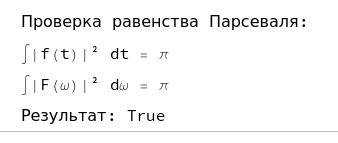
\includegraphics[width=\linewidth]{images/3P11.png}
  \captionof{\( (a, b) = (1, 1) \)}
\end{minipage}
\hfill
\begin{minipage}{0.32\textwidth}
  \centering
  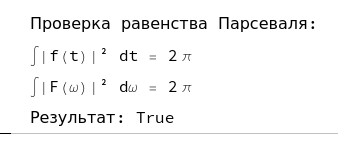
\includegraphics[width=\linewidth]{images/3P22.png}
  \captionof{\( (a, b) = (2, 2) \)}
\end{minipage}
\hfill
\begin{minipage}{0.32\textwidth}
  \centering
  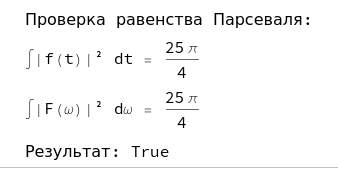
\includegraphics[width=\linewidth]{images/3P54.png}
  \captionof{\( (a, b) = (5, 4) \)}
\end{minipage}
\end{center}

\subsection{Функция Гаусса}
\subsubsection{Аналитика}
Исходная функция:
\[
f(t) = a \cdot e^{-b t^2}.
\]

Фурье-образ функции \( f(t) \):

\[
\hat{f}(\omega) = \int_{-\infty}^{\infty} f(t) e^{-i \omega t} \, dt = a \cdot \sqrt{\frac{\pi}{b}} \cdot e^{-\frac{\omega^2}{4b}},
\]

где \( a \) и \( b \) — параметры функции Гаусса, определяющие её амплитуду и ширину.


\subsubsection{Код}
\begin{lstlisting}[caption=Фурье-образ Гауссовой функции и проверка равенства Парсеваля]
f[t_, a_, b_] := a Exp[-b t^2]

a = 2;
b = 1;

fourier = FourierTransform[f[t, a, b], t, w]

Plot[f[t, a, b], {t, -5, 5}, PlotRange -> All, PlotStyle -> Thick, 
 AxesLabel -> {"t", "f(t)"}, PlotLabel -> "Функция Гаусса"]

Plot[Re[fourier], {w, -10, 10}, PlotRange -> All, PlotStyle -> Thick, 
 AxesLabel -> {"\[Omega]", "F(\[Omega])"}, 
 PlotLabel -> "Фурье-образ функции Гаусса"]

energyTimeDomain = 
 Integrate[Abs[f[t, a, b]]^2, {t, -Infinity, Infinity}]

energyFrequencyDomain = 
 Integrate[Abs[fourier]^2, {w, -Infinity, Infinity}]

Print["\nПроверка равенства Парсеваля:"]
Print["\[Integral]|f(t)|\.b2 dt = ", energyTimeDomain]
Print["\[Integral]|F(\[Omega])|\.b2 d\[Omega] = ", \
energyFrequencyDomain]
Print["Результат: ", energyTimeDomain == energyFrequencyDomain]
\end{lstlisting}
Этот код определяет функцию Гаусса, вычисляет ее Фурье-образ, строит графики и проверяет равенство Парсеваля.





\subsubsection{Вывод}
Теперь посмотрим на вывод кода. Я построю графики функции Гаусса и Фурье-образа для выбранных значений.
\begin{center}
\begin{minipage}{0.48\textwidth}
  \centering
  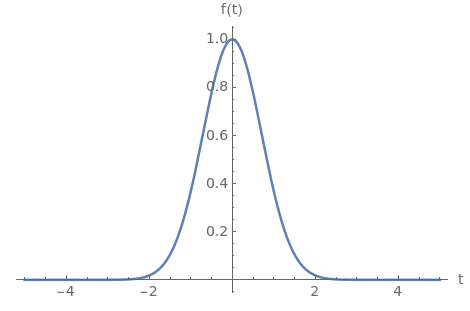
\includegraphics[width=\linewidth]{images/4f11.png}
  \captionof{\( f(t) \) для \( (a, b) = (1, 1) \) .}
\end{minipage}
\hfill
\begin{minipage}{0.48\textwidth}
  \centering
  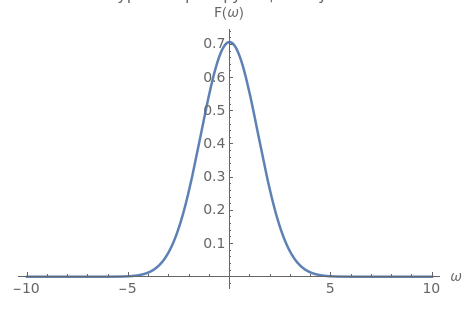
\includegraphics[width=\linewidth]{images/4F11.png}
  \captionof{\( \hat{f}(\omega) \) для \( (a, b) = (1, 1) \).}
\end{minipage}
\end{center}


\begin{center}
\begin{minipage}{0.48\textwidth}
  \centering
  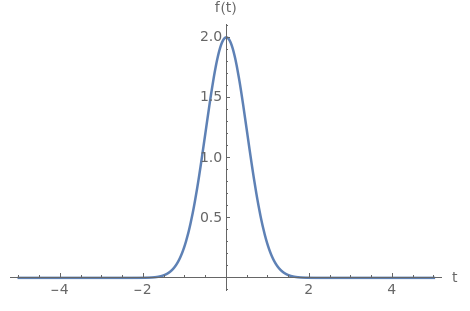
\includegraphics[width=\linewidth]{images/4f22.png}
  \captionof{\( f(t) \) для \( (a, b) = (2, 2) \) .}
\end{minipage}
\hfill
\begin{minipage}{0.48\textwidth}
  \centering
  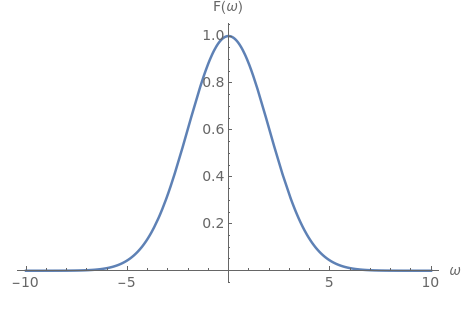
\includegraphics[width=\linewidth]{images/4F22.png}
  \captionof{\( \hat{f}(\omega) \) для \( (a, b) = (2, 2) \).}
\end{minipage}
\end{center}


\begin{center}
\begin{minipage}{0.48\textwidth}
  \centering
  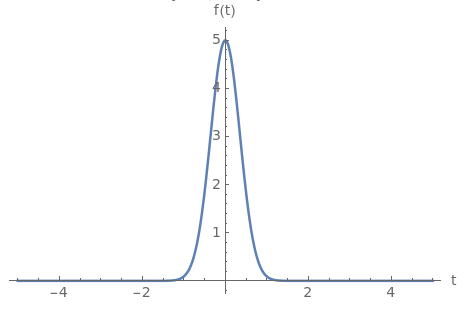
\includegraphics[width=\linewidth]{images/4f54.png}
  \captionof{\( f(t) \) для \( (a, b) = (5, 4) \) .}
\end{minipage}
\hfill
\begin{minipage}{0.48\textwidth}
  \centering
  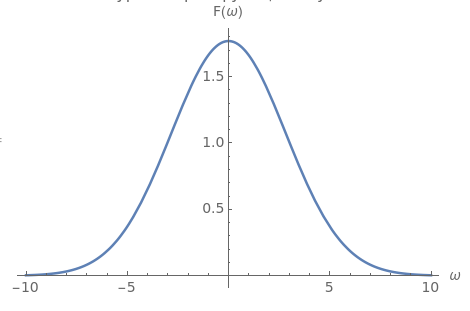
\includegraphics[width=\linewidth]{images/4F54.png}
  \captionof{\( \hat{f}(\omega) \) для \( (a, b) = (5, 4) \).}
\end{minipage}
\end{center}

Функция \( f(t) = a \cdot e^{-b t^2} \) имеет Фурье-образ, который также является функцией Гаусса. Параметр \( a \) влияет на амплитуду функции и её Фурье-образа: при увеличении \( a \) амплитуда Фурье-образа увеличивается пропорционально, потому что преобразование Фурье линейно, и умножение функции на константу \( a \) приводит к умножению её Фурье-образа на ту же константу.

Параметр \( b \) влияет на ширину функции Гаусса во временной области: при увеличении \( b \) функция становится более "узкой" (быстрее затухает), потому что экспонента \( e^{-b t^2} \) убывает быстрее. Это приводит к "расширению" её Фурье-образа в частотной области, потому что преобразование Фурье сохраняет энергию сигнала, и сжатие во временной области компенсируется расширением в частотной области.

Таким образом, при увеличении \( b \) Фурье-образ становится более широким, потому что сжатие функции во временной области приводит к расширению её спектра в частотной области, а при уменьшении \( b \) — более узким, потому что расширение функции во временной области приводит к сжатию её спектра в частотной области.\\


Также в моем коде присутствует проверка равенства Парсерваля. Для любых \( (a, b) \) проверка вернула \( True\) следовательно равенство выполнено.

\begin{center}
\begin{minipage}{0.32\textwidth}
  \centering
  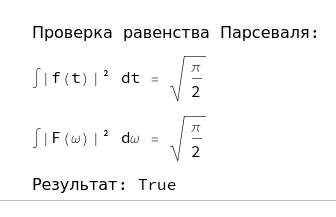
\includegraphics[width=\linewidth]{images/4P11.png}
  \captionof{\( (a, b) = (1, 1) \)}
\end{minipage}
\hfill
\begin{minipage}{0.32\textwidth}
  \centering
  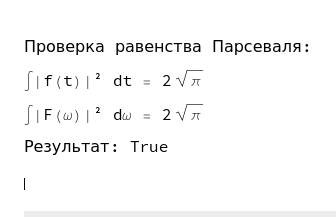
\includegraphics[width=\linewidth]{images/4P22.png}
  \captionof{\( (a, b) = (2, 2) \)}
\end{minipage}
\hfill
\begin{minipage}{0.32\textwidth}
  \centering
  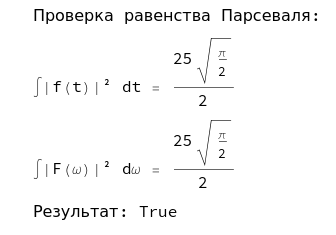
\includegraphics[width=\linewidth]{images/4P54.png}
  \captionof{\( (a, b) = (5, 4) \)}
\end{minipage}
\end{center}


\subsection{Двустороннее затухание}
\subsubsection{Аналитика}

Исходная функция:
\[
f(t) = a \cdot e^{-b |t|}.
\]

Фурье-образ вычисляется по формуле:
\[
\hat{f}(\omega) = \frac{1}{\sqrt{2\pi}} \int_{-\infty}^{\infty} a e^{-b |t|} e^{-i\omega t} \, dt = \frac{a}{\sqrt{2\pi}} \left( \int_{-\infty}^{0} e^{(b - i\omega) t} \, dt + \int_{0}^{\infty} e^{-(b + i\omega) t} \, dt \right).
\]

\[
\int_{-\infty}^{0} e^{(b - i\omega) t} \, dt = \left[ \frac{e^{(b - i\omega) t}}{b - i\omega} \right]_{-\infty}^{0} = \frac{1}{b - i\omega},
\]
\[
\int_{0}^{\infty} e^{-(b + i\omega) t} \, dt = \left[ \frac{e^{-(b + i\omega) t}}{-(b + i\omega)} \right]_{0}^{\infty} = \frac{1}{b + i\omega}.
\]

\[
\hat{f}(\omega) = \frac{a}{\sqrt{2\pi}} \left( \frac{1}{b - i\omega} + \frac{1}{b + i\omega} \right) = \frac{a}{\sqrt{2\pi}} \cdot \frac{2b}{b^2 + \omega^2}.
\]

Таким образом, Фурье-образ функции двустороннего затухания:
\[
\hat{f}(\omega) = \frac{2ab}{\sqrt{2\pi} (b^2 + \omega^2)}.
\]


Для параметров \( (a, b) = (1, 1) \):
\[
\hat{f}(\omega) = \frac{2}{\sqrt{2\pi} (1 + \omega^2)}.
\]

Для параметров \( (a, b) = (2, 2) \):
\[
\hat{f}(\omega) = \frac{8}{\sqrt{2\pi} (4 + \omega^2)}.
\]

Для параметров \( (a, b) = (5, 4) \):
\[
\hat{f}(\omega) = \frac{40}{\sqrt{2\pi} (16 + \omega^2)}.
\]

\subsubsection{Код}
\begin{lstlisting}[caption=Фурье-образ двустороннего затухания и проверка равенства Парсеваля]
f[t_, a_, b_] := a Exp[-b Abs[t]]

a = 1;
b = 2;

fourier = FourierTransform[f[t, a, b], t, w]

Plot[f[t, a, b], {t, -5, 5}, PlotRange -> All, PlotStyle -> Thick, 
 AxesLabel -> {"t", "f(t)"}, 
 PlotLabel -> "Функция с двусторонним затуханием"]

Plot[Re[fourier], {w, -10, 10}, PlotRange -> All, PlotStyle -> Thick, 
 AxesLabel -> {"\[Omega]", "F(\[Omega])"}, 
 PlotLabel -> "Фурье-образ функции с двусторонним затуханием"]

energyTimeDomain = 
 Integrate[Abs[f[t, a, b]]^2, {t, -Infinity, Infinity}]

energyFrequencyDomain = 
 Integrate[Abs[fourier]^2, {w, -Infinity, Infinity}]

Print["\nПроверка равенства Парсеваля:"]
Print["\[Integral]|f(t)|\.b2 dt = ", energyTimeDomain]
Print["\[Integral]|F(\[Omega])|\.b2 d\[Omega] = ", \
energyFrequencyDomain]
Print["Результат: ", energyTimeDomain == energyFrequencyDomain]
\end{lstlisting}
Этот код определяет функцию двустороннего затухания, вычисляет ее Фурье-образ, строит графики и проверяет равенство Парсеваля.


\subsubsection{Вывод}
Теперь посмотрим на вывод кода. Я построю графики функции двустороннего затухания и Фурье-образа для выбранных значений.
\begin{center}
\begin{minipage}{0.48\textwidth}
  \centering
  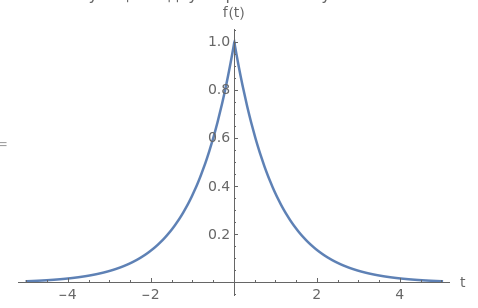
\includegraphics[width=\linewidth]{images/5f11.png}
  \captionof{\( f(t) \) для \( (a, b) = (1, 1) \) .}
\end{minipage}
\hfill
\begin{minipage}{0.48\textwidth}
  \centering
  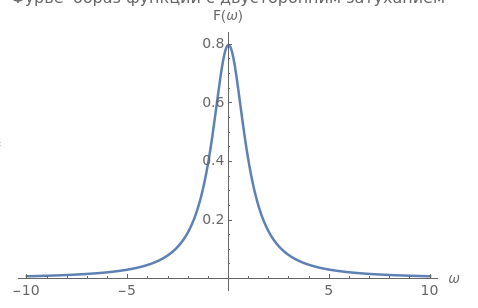
\includegraphics[width=\linewidth]{images/5F11.png}
  \captionof{\( \hat{f}(\omega) \) для \( (a, b) = (1, 1) \).}
\end{minipage}
\end{center}


\begin{center}
\begin{minipage}{0.48\textwidth}
  \centering
  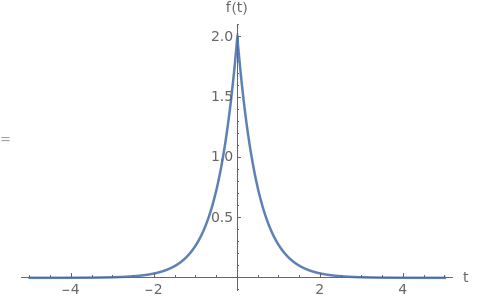
\includegraphics[width=\linewidth]{images/5f22.png}
  \captionof{\( f(t) \) для \( (a, b) = (2, 2) \) .}
\end{minipage}
\hfill
\begin{minipage}{0.48\textwidth}
  \centering
  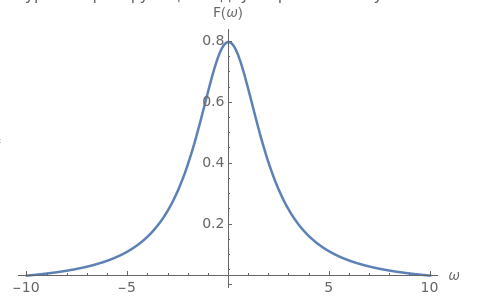
\includegraphics[width=\linewidth]{images/5F22.png}
  \captionof{\( \hat{f}(\omega) \) для \( (a, b) = (2, 2) \).}
\end{minipage}
\end{center}


\begin{center}
\begin{minipage}{0.48\textwidth}
  \centering
  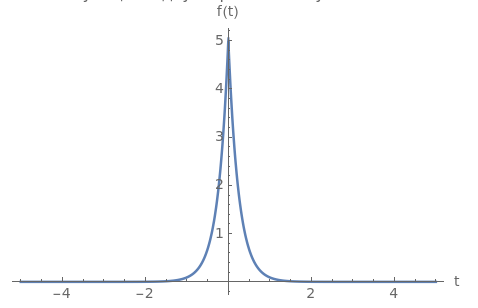
\includegraphics[width=\linewidth]{images/5f54.png}
  \captionof{\( f(t) \) для \( (a, b) = (5, 4) \) .}
\end{minipage}
\hfill
\begin{minipage}{0.48\textwidth}
  \centering
  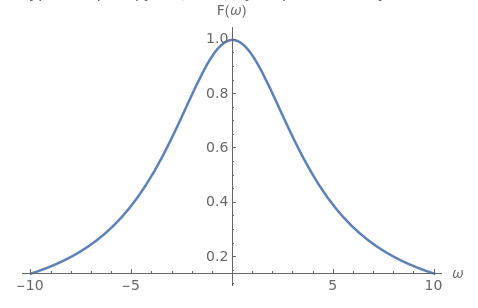
\includegraphics[width=\linewidth]{images/5F54.png}
  \captionof{\( \hat{f}(\omega) \) для \( (a, b) = (5, 4) \).}
\end{minipage}
\end{center}

Функция \( f(t) = a \cdot e^{-b |t|} \) имеет Фурье-образ, который определяется свойствами преобразования Фурье. Параметр \( a \) влияет на амплитуду функции и её Фурье-образа: при увеличении \( a \) амплитуда Фурье-образа увеличивается пропорционально, потому что преобразование Фурье линейно, и умножение функции на константу \( a \) приводит к умножению её Фурье-образа на ту же константу.

Параметр \( b \) влияет на скорость затухания функции: при увеличении \( b \) функция становится более "узкой" (быстрее затухает), потому что экспонента \( e^{-b |t|} \) убывает быстрее. Это приводит к "расширению" её Фурье-образа в частотной области, потому что преобразование Фурье сохраняет энергию сигнала, и сжатие во временной области компенсируется расширением в частотной области.

Таким образом, при увеличении \( b \) Фурье-образ становится более широким, потому что сжатие функции во временной области приводит к расширению её спектра в частотной области, а при уменьшении \( b \) — более узким, потому что расширение функции во временной области приводит к сжатию её спектра в частотной области. \\


Также в моем коде присутствует проверка равенства Парсерваля. Для любых \( (a, b) \) проверка вернула \( True\) следовательно равенство выполнено.

\begin{center}
\begin{minipage}{0.32\textwidth}
  \centering
  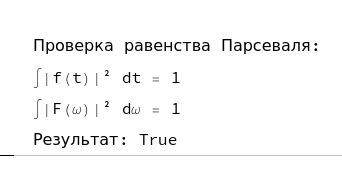
\includegraphics[width=\linewidth]{images/5P11.png}
  \captionof{\( (a, b) = (1, 1) \)}
\end{minipage}
\hfill
\begin{minipage}{0.32\textwidth}
  \centering
  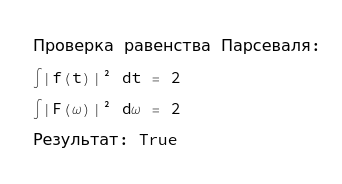
\includegraphics[width=\linewidth]{images/5P22.png}
  \captionof{\( (a, b) = (2, 2) \)}
\end{minipage}
\hfill
\begin{minipage}{0.32\textwidth}
  \centering
  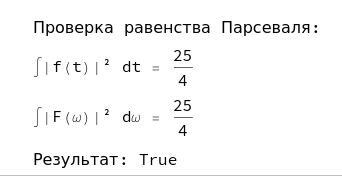
\includegraphics[width=\linewidth]{images/5P54.png}
  \captionof{\( (a, b) = (5, 4) \)}
\end{minipage}
\end{center}

\section{Комплексное задание}
\subsection{Краткое условие}
Выбрать одну функцию \( f(t) \) из задания 1 и один набор параметров \( a, b \). Рассмотреть сдвинутую функцию \( g(t) = f(t + c) \) и провести исследование её Фурье-образа \(\beta(\omega)\):

\begin{itemize}
    \item Привести аналитическое выражение для Фурье-образа \(\beta(\omega)\).

    \item Выбрать три значения параметра \( c \neq 0 \) и построить графики \( g(t) \). Проанализировать влияние \( c \) на оригинал функции.

    \item Для выбранных значений \( c \) построить:
    \begin{itemize}
        \item Графики вещественной и мнимой компонент Фурье-образа: \( \text{Re}(\beta(\omega)) \) и \( \text{Im}(\beta(\omega)) \).
        \item График модуля Фурье-образа: \( |\beta(\omega)| \).
    \end{itemize}

    \item Проанализировать влияние параметра \( c \) на компоненты и модуль Фурье-образа.

    \item Сделать выводы.
\end{itemize}




\subsection{Аналитика}


Рассмотрим функцию \( f(t) = a e^{-b |t|} \), где \( a = 1 \) и \( b = 1 \). Определим сдвинутую функцию \( g(t, c) = f(t + c) \), где \( c \) принимает значения из набора \( c = \{1, 2, 3\} \). Тогда:

\[
g(t, c) = a e^{-b |t + c|}.
\]

Фурье-образ функции \( g(t, c) \) вычисляется следующим образом:
\[
\hat{g}(\omega, c) = {F}\{g(t, c)\}(\omega) = \int_{-\infty}^{\infty} a e^{-b |t + c|} e^{-i \omega t} \, dt.
\]

Используя свойство сдвига Фурье-преобразования, получаем:
\[
\hat{g}(\omega, c) = e^{i \omega c} \cdot {F}\{f(t)\}(\omega).
\]

Фурье-образ исходной функции \( f(t) = a e^{-b |t|} \) известен и равен:
\[
\hat{f}(\omega) = \frac{2a b}{b^2 + \omega^2}.
\]

Таким образом, Фурье-образ сдвинутой функции \( g(t, c) \) выражается как:
\[
\hat{g}(\omega, c) = e^{i \omega c} \cdot \frac{2a b}{b^2 + \omega^2}.
\]






















\subsection{Код}
\begin{lstlisting}
a = 1;
b = 1;
f[t_] := a Exp[-b Abs[t]];

cValues = {1, 2, 3};
g[t_, c_] := f[t + c];

fourierTransforms = 
  Table[FourierTransform[g[t, c], t, \[Omega]], {c, cValues}];

Plot[Evaluate[Table[g[t, c], {c, cValues}]], {t, -10, 5}, 
 PlotLabel -> "Графики g(t) для c = {1, 2, 3}", 
 PlotLegends -> Table["c = " <> ToString[c], {c, cValues}], 
 PlotRange -> {Automatic, {0, 1}}]

plotsReIm = 
 Table[Plot[{Re[fourierTransforms[[c]]], 
    Im[fourierTransforms[[c]]]}, {\[Omega], -10, 10}, 
   PlotLegends -> {"Re(g(\[Omega]))", "Im(g(\[Omega]))"}, 
   PlotLabel -> 
    "Re и Im Фурье-образа для c = " <> ToString[cValues[[c]]]], {c, 
   Length[cValues]}]

plotsAbs = 
 Plot[Evaluate[
   Table[Abs[fourierTransforms[[c]]], {c, 
     Length[cValues]}]], {\[Omega], -10, 10}, 
  PlotLabel -> "Модуль Фурье-образа для c = {1, 2, 3}", 
  PlotLegends -> 
   Table["c = " <> ToString[cValues[[c]]], {c, Length[cValues]}]]
\end{lstlisting}

Код задаёт \( a = 1 \), \( b = 1 \), \( c = \{1, 2, 3\} \) и функцию \( f(t) = 2e^{-2|t|} \). Для \( g(t, c) = f(t + c) \) вычисляет Фурье-образы и строит графики \( g(t, c) \), действительной и мнимой частей Фурье-образа, а также их модуля.






















\subsection{Вывод}
Теперь посмотрим и проанализируем графики, которые выдал мой код. В этом задании, я решила не делать много картинок и что было целесообразно нарисовала на одном графике.
\begin{figure}[H]
    \centering
    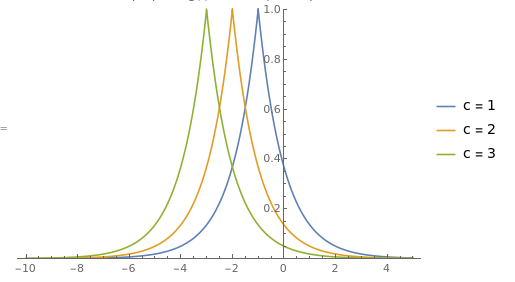
\includegraphics[width=0.5\textwidth]{images/g(t).png}
    \caption{\( g(t)\) для \( c = \{1, 2, 3\} \)} % Подпись без номера
    \label{fig:g_t}
\end{figure}

\begin{figure}[H]
    \centering
    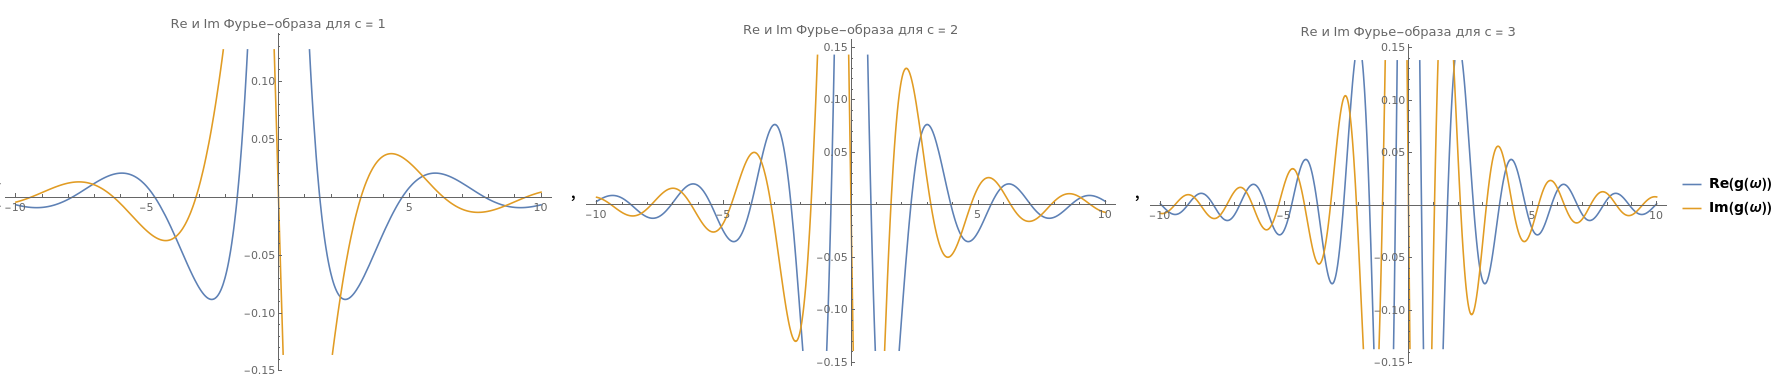
\includegraphics[width=1.1\textwidth]{images/ReIm.png}
    \caption{\( Re \) и \( Im \) Фурье-образа для \( c = \{1, 2, 3\} \)} % Подпись без номера
    \label{fig:ReIm}
\end{figure}

\begin{figure}[H]
    \centering
    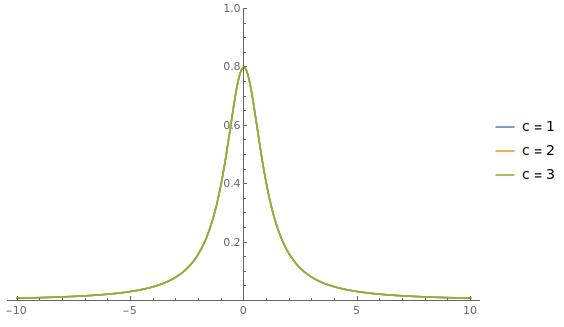
\includegraphics[width=0.5\textwidth]{images/Abs.png}
    \caption{Модуль Фурье-образа для \( c = \{1, 2, 3\} \)} % Подпись без номера
    \label{fig:Abs}
\end{figure}

Анализ показывает, что амплитуды действительной и мнимой частей Фурье-образа сохраняются при сдвиге \( c \), так как сдвиг влияет только на фазу, но не на амплитуду. Это следует из свойства Фурье-преобразования:
\[
\hat{g}_c(\omega) = e^{i \omega c} \cdot \hat{g}(\omega),
\]
где \( e^{i \omega c} \) — фазовый множитель. С увеличением \( |c| \) частота колебаний \(\operatorname{Re} \hat{g}(\omega)\) и \(\operatorname{Im} \hat{g}(\omega)\) возрастает, что связано с линейным изменением фазы.

Знак \( c \) определяет положение мнимой части: при \( c > 0 \) она смещается вправо. Действительная часть остаётся симметричной, так как Фурье-образ действительной функции имеет чётную действительную часть.

Модуль Фурье-образа инвариантен относительно сдвигов. Его форма совпадает с модулем Фурье-образа несдвинутой функции.


\newpage
\section{Музыкальное задание}
\subsection{Краткое условие}

Требуется:
\begin{itemize}
    \item Преобразовать запись музыкального аккорда в массив \( f(t) \).
    \item Построить график \( f(t) \).
    \item Найти Фурье-образ \( f(\nu) \) с помощью численного интегрирования
    \item Построить график модуля Фурье-образа \( |f(\nu)| \).
    \item Определить основные частоты и соотнести их с музыкальными нотами.
\end{itemize}

Для этого задания я выбрала 22 запись.
\subsection{Код}








Данный код выполняет анализ аудиосигнала, загруженного из файла в формате \texttt{.wav}. Основные этапы анализа включают построение графиков во временной и частотной областях, а также поиск основных частот в сигнале.


Функция \texttt{load\_audio} загружает аудиофайл и извлекает данные и частоту дискретизации.

Функция \texttt{plot\_time\_domain} строит график амплитуды сигнала в зависимости от времени:
\[
f(t) = \text{Амплитуда сигнала}
\]

Функция \texttt{compute\_fourier\_transform} вычисляет преобразование Фурье для перехода в частотную область:
\[
F(\nu) = \frac{1}{N} \sum_{k=0}^{N-1} f(k) e^{-i 2 \pi \nu k / N}
\]
где \( N \) — количество отсчётов, \( \nu \) — частота.

Функция \texttt{plot\_frequency\_domain} строит график амплитуды спектра в зависимости от частоты:
\[
|F(\nu)| = \text{Амплитуда спектра}
\]

Функция \texttt{find\_peak\_frequencies} находит основные частоты в спектре сигнала, используя метод поиска пиков.


\begin{lstlisting}[language=Python, caption=Обработка аудиосигнала с использованием преобразования Фурье]
import numpy as np
import matplotlib.pyplot as plt
from scipy.io.wavfile import read
from scipy.signal import find_peaks

def load_audio(file_path):
    sample_rate, audio_data = read(file_path)
    if len(audio_data.shape) > 1:
        audio_data = audio_data[:, 0]
        return sample_rate, audio_data

def plot_time_domain(sample_rate, audio_data):
    time = np.arange(0, len(audio_data)) / sample_rate
    plt.figure(figsize=(10, 4))
    plt.plot(time, audio_data)
    plt.title("График f(t)")
    plt.xlabel("Время (с)")
    plt.ylabel("Амплитуда")
    plt.grid()
    plt.show()

def compute_fourier_transform(audio_data, sample_rate):
    n = len(audio_data)
    frequencies = np.fft.fftfreq(n, d=1/sample_rate)
    fourier_transform = np.fft.fft(audio_data) / n
    return frequencies[:n // 2], fourier_transform[:n // 2]

def plot_frequency_domain(frequencies, fourier_transform):
    plt.figure(figsize=(10, 4))
    plt.plot(frequencies, np.abs(fourier_transform))
    plt.title("График |f(ν)|")
    plt.xlabel("Частота (Гц)")
    plt.ylabel("Амплитуда")
    plt.grid()
    plt.show()

def find_peak_frequencies(frequencies, fourier_transform, num_peaks=3):
    peaks, _ = find_peaks(np.abs(fourier_transform), height=np.max(np.abs(fourier_transform)) * 0.1)
    peak_indices = np.argsort(np.abs(fourier_transform[peaks]))[-num_peaks:]
    return frequencies[peaks[peak_indices]]

def main(file_path):
    sample_rate, audio_data = load_audio(file_path)
    plot_time_domain(sample_rate, audio_data)
    frequencies, fourier_transform = compute_fourier_transform(audio_data, sample_rate)
    plot_frequency_domain(frequencies, fourier_transform)
    peak_frequencies = find_peak_frequencies(frequencies, fourier_transform)
    print("Основные частоты:", peak_frequencies)

if __name__ == "__main__":
    file_path = "/home/eva/Документы/itmo/2_course/chMetods/lab2/audio.wav"
    main(file_path)
\end{lstlisting}


\subsection{Вывод}
А теперь посмотрим, что за графики и частоты вывел мой код.
\begin{lstlisting}[language=Python, caption=Вывод основных частот аккорды]
Основные частоты: [329.38063667 261.53756019 440.2298894 ]
\end{lstlisting}

Частоты 329.38 Гц, 261.54 Гц и 440.23 Гц соответствуют аккорду Ля-минор.

Аккорд состоит из нот:
\begin{itemize}
    \item Ля (A): 440.23 Гц
    \item До (C): 261.54 Гц
    \item Ми (E): 329.38 Гц
\end{itemize}










\begin{figure}[h!]
    \centering
    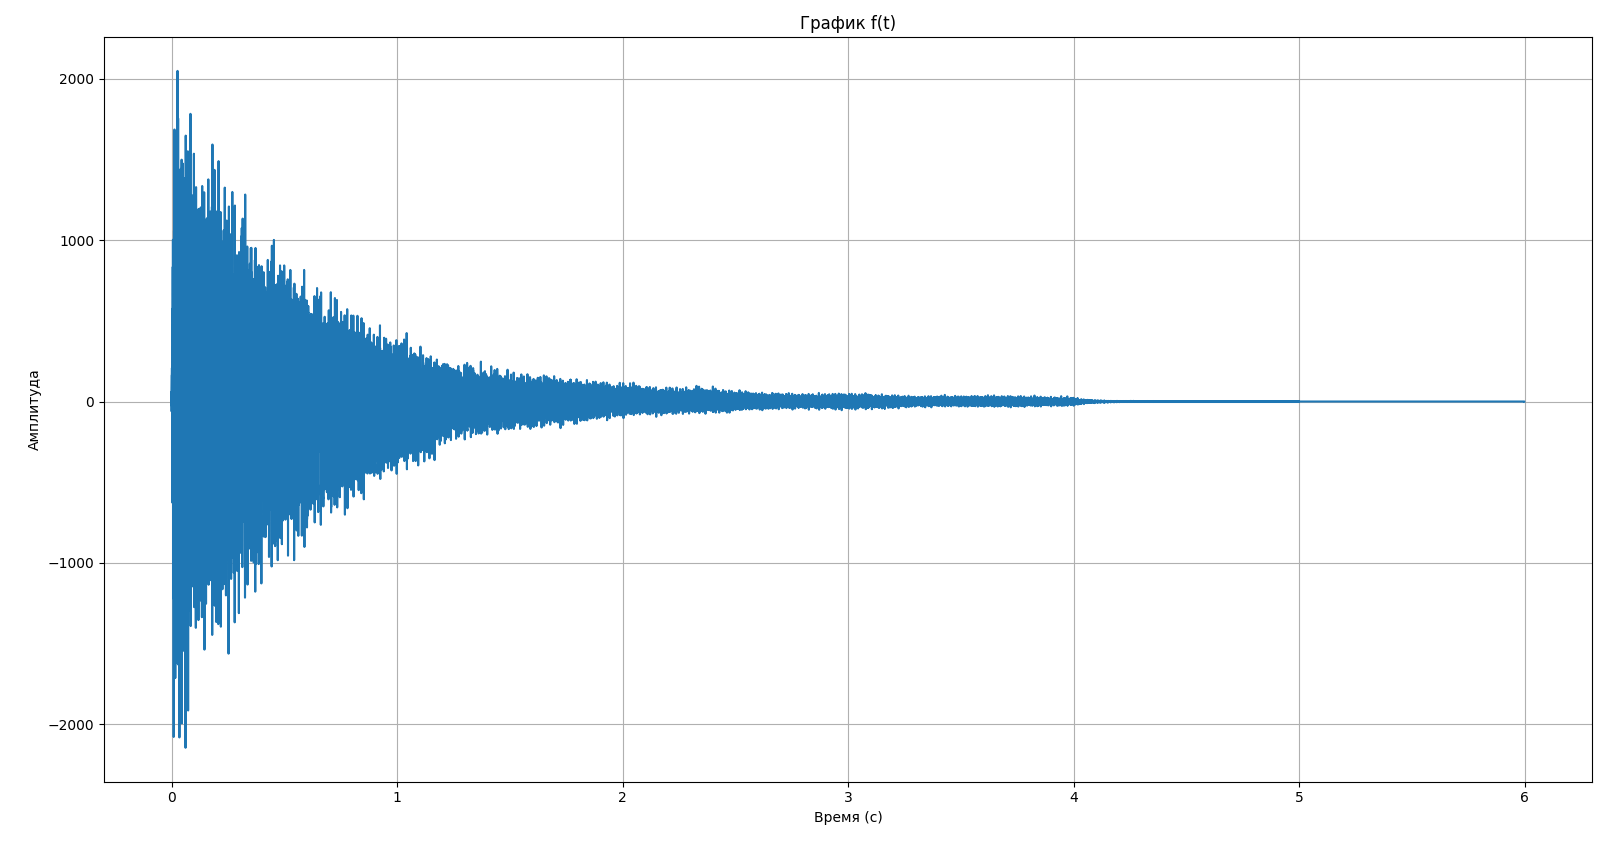
\includegraphics[width=0.7\textwidth]{images/f(t).png}
    \caption{График амплитуды от времени} % Подпись без номера
    \label{fig:ReIm}
\end{figure}

\begin{figure}[h!]
    \centering
    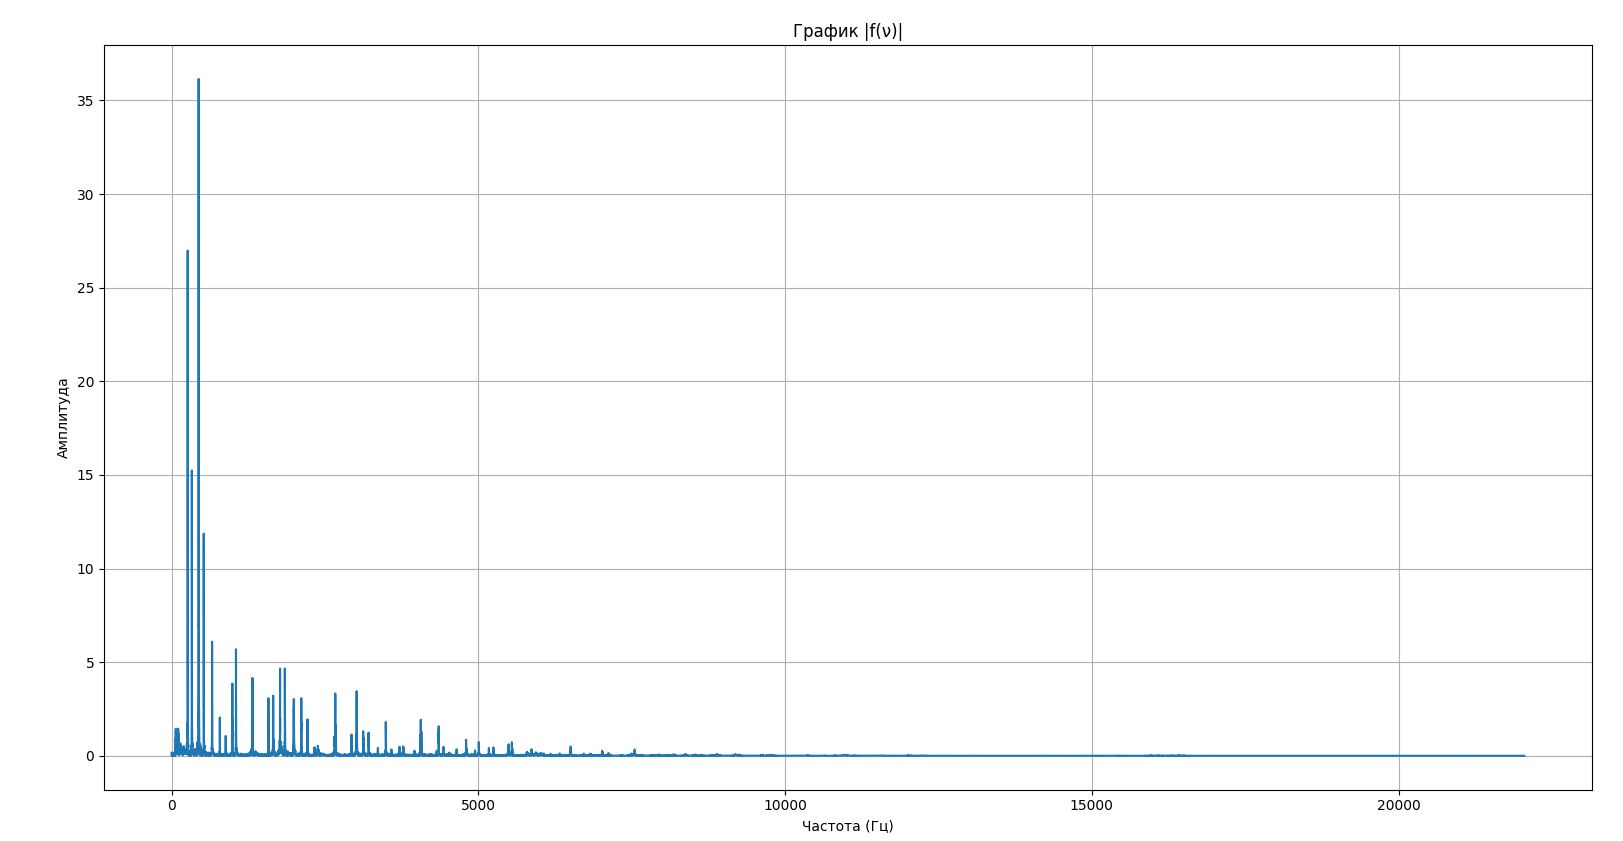
\includegraphics[width=0.7\textwidth]{images/f(v).png}
    \caption{Модуль Фурье-образа звука} % Подпись без номера
    \label{fig:Abs}
\end{figure}






\newpage
\section{Примечания}

\begin{itemize}
    \item Для заданий 1, 2 был использован язык \texttt{Wolfram Matematica}, 3 задание написано на \texttt{python}.
    \item Репозиторий \href{https://github.com/decadeos/frequency-methods}{github} сисходным кодом и tex-проектом.
\end{itemize}





\end{document}
